\documentclass[twocolumn,twoside,10pt,a4paper]{article}

\usepackage[english]{babel}  % portuguese
\usepackage{graphicx}           % images: .png or .pdf w/ pdflatex; .eps w/ latex

%% For iso-8859-1 (latin1), comment next line and uncomment the second line
\usepackage[utf8]{inputenc}

\usepackage{times}              % PS fonts
\usepackage[T1]{fontenc}        % T1 fonts
%\usepackage{lastpage}           % to have lastpage in headers
\usepackage{url}                % urls

% geometry package
\usepackage[outer=20mm,inner=30mm,vmargin=20mm,includehead,includefoot,headheight=15pt]{geometry}

%% space between columns
\columnsep 10mm

% avoid widows and orphans
\clubpenalty=300
\widowpenalty=300

\usepackage{listings}
\lstdefinestyle{xml}{
	language=XML,
	extendedchars=true,
	inputencoding=latin1,
	tabsize=4,
	showstringspaces=false,
	basicstyle=\scriptsize,
	keywordstyle=\ttfamily\color{blue},
	stringstyle=\ttfamily\color{orange},
	identifierstyle=\ttfamily,
	commentstyle=\ttfamily\color{darkred},
	morecomment=[s][\ttfamily\color{javadoc}]{/**}{*/},
	numbers=left
}

\usepackage[pdftex]{hyperref}
\hypersetup{%
    a4paper = true,              % use A4 paper
    bookmarks = true,            % make bookmarks
    colorlinks = true,           % false: boxed links; true: colored links
    pdffitwindow = false,        % page fit to window when opened
    pdfpagemode = UseNone,       % do not show bookmarks
    pdfpagelayout = SinglePage,  % displays a single page
    pdfpagetransition = Replace, % page transition
    linkcolor=blue,              % hyperlink colors
    urlcolor=blue,
    citecolor=blue,
    anchorcolor=green
}

\usepackage{indentfirst}       % indent also 1st paragraph

\pagestyle{myheadings}         % Option to put page headers
\markboth{{\small\it xml2json}}
{{\small\it Group 08, \today}}

%\hyphenation{}                  % explicit hyphenation

% entities
\newcommand{\class}[1]{{\normalfont\slshape #1\/}}

\title{xml2json}

\author{João Gradim\\
\small Faculdade de Engenharia da Universidade do Porto,\\[-0.8ex]
\small R.\ Dr.\ Roberto Frias, 4200-465 Porto\\[-0.8ex]
\small \texttt{ei05030@fe.up.pt}\\
\and
Nuno Polónia\\
\small Faculdade de Engenharia da Universidade do Porto,\\[-0.8ex]
\small R.\ Dr.\ Roberto Frias, 4200-465 Porto\\[-0.8ex]
\small \texttt{ei05037@fe.up.pt}
}

\date{\today}

\begin{document}

\maketitle
\thispagestyle{plain}

\begin{abstract}

\end{abstract}

\section{Introduction}\label{sec:intro}
On the newly programmable Web, mashups are flourishing. Designers create mashups by combining components of existing Web sites and applications \cite{maximilien}. The complexity and usefulness of web services has been increasing exponentially making them emerge as a major technology for companies and individuals \cite{benslimane}.

This exchange of data and functionalities between web services is powered by API's which are abstract interfaces to the applications. They usually receive HTTP requests and return the information in an XML dialect.

With the incredible advances on Javascript Engines rendering speeds and the extensive use of AJAX by web applications, JSON is becoming the prefered API output language by developers mainly because it corresponds to a native Javascript object.

However, some of the most used website APIs only provide output in an custom XML dialect. As such, the main objective of this project is to create a web application that acts as a proxy for any XML API, transforming the XML output into JSON.

\section{Application}\label{sec:application}

%The project consists of a web application that allows an user transform an XML document to a JSON representation. It provides statistics about the requested APIs, a live editor that allows

\subsection{User Requirements}\label{sec:user-requirements}

\begin{itemize}
    \item The user should be able to transform any XML document to a valid JSON representation
    \item The user should be able to transform XML to JSON visually (in a compatible browser) or programmatically (through an HTTP GET request)
    \item The system should provide a live XML to JSON editor, so that the user is able preview the result of a transformation
    \item The system should provide statistics about the requested APIs
    \item The system should be able to recover from errors, informing the user about the error and how it can recover from it
\end{itemize}

\subsection{Similar Projects}\label{sec:similar-projects}

Most modern programming languages (such as Ruby and Python) provide support for both XML and JSON formats, either built-in or with 3rd-party libraries, and allow programmers to easily convert between these representations. However, there is not an universal, language-agnostic service that allows programmers to easily convert an XML document to a JSON representation, that ensures that the transformation does not change with the programming language used.

\subsection{Architecture}\label{sec:architecture}

As previously stated, xml2json acts primarily as a proxy that transforms an XML document to a JSON representation. As such, a user may perform a GET request to the xml2json api converter url \footnote{at the moment of writing, \url{http://xml2json.ath.cx/convert.json}}, specifying the \verb!request-url! parameter --- which corresponds to the location of the XML document they wish to convert to JSON. The application then makes a request to whichever address the user specified in \verb!request-url!, retrieves the XML document, converts it to JSON and finally responds to the user with the JSON representation of the specified XML document. While performing the transformation, the system also saves the access to the database in order to keep track of which APIs have been accessed.

Figure \ref{fig:system_arch} represents this architecture.

\begin{figure}[h]
    \centering
    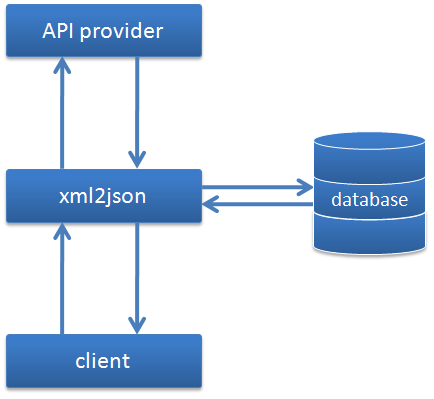
\includegraphics[width=80mm]{images/arch.png}
    \caption{System Architecture}
    \label{fig:system_arch}
\end{figure}

\subsection{Implementation}\label{sec:implementation}

The application was implemented using the Ruby programming language and the Ruby on Rails framework for the backend, and HTML5, CSS 2/3 and JavaScript for the frontend.

\subsubsection{XSLT Transformation}\label{sec:xslt-transformation}

There are two methods used to apply the transformation to the XML: for the api converter, the transformation is processed at the application level, using Ruby and libxml to apply the xml2json stylesheet to an arbitrary XML document. For the live editor, as it would be very costly and inneficient to make a request to the application each time the text on the editor changed, a different approach had to be taken: by taking advantage of the \verb!XSLTProcessor! JavaScript object, it's possible to delegate the transformation to the client's browser, providing a much better response while not overloading the server with requests.

\section{Results}\label{sec:results}
% ACHO QUE ISTO ESTÁ MAL EXPLICADO MAS ESTOU A TER DIFICULDADES EM EXPLICAR MELHOR
In order to overcome some quirks in the translation from XML to JSON some structural changes had to be made to maintain the data integrity.

The User Requirements for this application were completely fulfilled without any known bug in the translation of several API's output.

\section{Final Remarks}\label{sec:final-remarks}


\section{Future Work}\label{sec:future-work}

The next step will be to fully document all the idiosyncrasies of the XML translation into JSON and turn the statistics module into a monitoring module in order to get more data in bugs that might arise with the addition of newer APIs.

%% auto bibliographic list
\renewcommand{\bibname}{References}
\bibliographystyle{unsrt-pt}
\bibliography{lapd3}

\end{document}

